\documentclass{article}

\usepackage{tabularx}
\usepackage[table]{xcolor}
\usepackage{hyperref}
\usepackage{cleveref}
\usepackage{tikz}
\usetikzlibrary{positioning, calc, shapes, arrows, fit}
\usepackage{circuitikz}
\usepackage{subcaption}
\usepackage[colorinlistoftodos]{todonotes}
\linespread{0.9}
\hypersetup{
    colorlinks = true,
    linkbordercolor = {black},
    linkcolor=black
}
\begin{document}
\title{Lab 1 -- Measuring ``Parasitics'' of Passive Components with a VNA}
\author{
    Yifan Zhu\\
    Lab Partner: John Kustin
}
\maketitle

\begin{abstract}
    S-Parameters of passive components are measured using a Vector Network Analyzer (VNA), and more realistic circuit models containing parasitics are proposed.
    The proposed circuit models are simulated in LTSPice, and compared against the experimentally obtained results.
\end{abstract}

\section{Introduction}
Real life passive components are far from ideal.
All capacitors, inductors, and resistors have some parasitic capacitance, inductance, and resistance.
But how can we measure these parasitics?
How can we build good electric models of these real-world components?
To this end, we use Vector Network Analyzers (VNA) to measure the frequency response of these passive components, use our understanding of circuit elements to conjecture about good circuit models, and use LTSpice to verify that the circuit models match what we observe.

\section{Experimental Setup}
\begin{figure}[h]
    \centering
    \begin{subfigure}{.5\linewidth}
        \centering
        \includegraphics[width=.8\linewidth]{./pics/test_loads.jpg}
        \caption{Picture of RF Demo Kit NWDZ}
        \label{fig:test_loads}
    \end{subfigure}%
    \begin{subfigure}{.5\linewidth}
        \centering
        \includegraphics[width=.8\linewidth]{./pics/NanoVNA.jpg}
        \caption{Picture of NanoVNA}
        \label{fig:nanovna}
    \end{subfigure}
    \caption{Picture of Tools used in Experiment}
\end{figure}

The passive components of interest are all surface mount components on the \emph{RF Demo Kit NWDZ Rev-01-10} (\Cref{fig:test_loads}), and
we use the NanoVNA (\Cref{fig:nanovna}) to perform the measurements.
Care is taken to calibrate the NanoVNA each time before use.

\section{Measurements and Results}

\subsection{Capacitor}
\begin{figure}[h]
    \centering
    \begin{subfigure}{0.5\linewidth}
        \includegraphics[width=\linewidth]{./pics/capacitor_meas_smith.png}
        \caption{S11 on Smith Chart}
    \end{subfigure}%
    \begin{subfigure}{0.5\linewidth}
        \includegraphics[width=\linewidth]{./pics/capacitor_meas_db.png}
        \caption{Magnitude of Impedance (in dBOmhs)}
    \end{subfigure}

    \begin{subfigure}{\linewidth}
        \centering
        \begin{tabular}{ |c|c|c|c| }
            \hline
            Frequency (MHz) & S11         & Impedance (Ohm)   & Comment
            \\\hline
            0.05            & 1.00-0.00j  & 1114.88-24861.18j & Close to DC
            \\\hline
            10.049          & 0.82-0.58j  & -0.17-157.00j     & Low Frequency (Capacitive Regime)
            \\\hline
            100.04          & -0.86-0.53j & -0.41-14.14j      & Low Frequency (Capacitive Regime)
            \\\hline
            304.020         & -0.99-0.00j & 0.14-0.03j        & Resonance Frequency
            \\\hline
            500             & -0.94+0.20j & 0.98+5.25j        & High Frequency (Inductive Regime)
            \\\hline
        \end{tabular}
        \caption{S11 and Impedance at selected frequencies}
        \label{tab:capacitor_meas}
    \end{subfigure}

    \caption{S Parameter of Measured Capacitor}
    \label{fig:capacitor_meas}
\end{figure}

We measured the S-Parameters of the capacitor in the kit (item 7 in \Cref{fig:test_loads}), and the results are depicted in \Cref{fig:capacitor_meas}.

\begin{figure}
    \centering
    \begin{subfigure}{.5\linewidth}
        \centering
        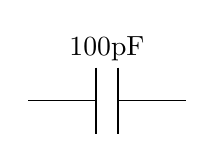
\begin{tikzpicture}
            \draw (0,0) to[C, label=100pF] ++(2,0);
        \end{tikzpicture}
        \caption{Ideal Capacitor Model}
        \label{fig:capacitor_c}
    \end{subfigure}%
    \begin{subfigure}{.5\linewidth}
        \centering
        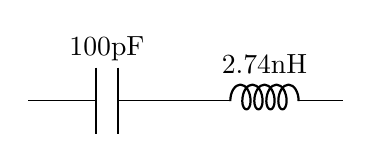
\begin{tikzpicture}
            \draw (0,0) to[C, label=100pF] ++(2,0)
            to[L, label=2.74nH] ++(2, 0);
        \end{tikzpicture}
        \caption{Capacitor with Series Inductance}
        \label{fig:capacitor_cl}
    \end{subfigure}%

    \begin{subfigure}{.5\linewidth}
        \centering
        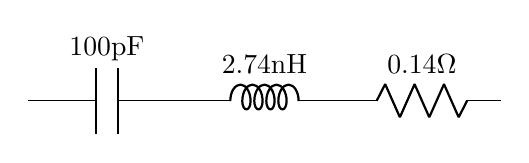
\begin{tikzpicture}
            \draw (0,0) to[C, label=100pF] ++(2,0)
            to[L, label=2.74nH] ++(2, 0)
            to[R, label=$0.14\Omega$] ++(2,0);
        \end{tikzpicture}
        \caption{Capacitor with Series Inductance and Resistance}
        \label{fig:capacitor_clr}
    \end{subfigure}%
    \caption{Electric Models of Real Life Capacitor}
\end{figure}

\begin{figure}
    \centering
    \begin{subfigure}{\linewidth}
        \centering
        \includegraphics[width=\linewidth]{./pics/capacitor_models_smith.png}
        \caption{S11 of electric models of capacitor on Smith Chart}
        \label{fig:capacitor_compare_s}
    \end{subfigure}

    \begin{subfigure}{\linewidth}
        \centering
        \includegraphics[width=\linewidth]{./pics/capacitor_models_db.png}
        \caption{Magnitude of Impedance of electric models of capacitor in dBOhms.}
        \label{fig:capacitor_compare_z}
    \end{subfigure}
    \caption{Electric Characteristics of real capacitor compared with various models}
    \label{fig:capacitor_compare}
\end{figure}

\subsubsection{Ideal Capacitor Model}

Using the impedance at 10MHz, we see that the capacitance is roughly
$$\frac{1}{2\pi\cdot 10MHz \cdot 157 \Omega} \approx 100pF .$$
So our first model of the element would just be an ideal capacitor of $100pF$ (\Cref{fig:capacitor_c}).

The circuit is simulated in LTSpice and results are shown in \Cref{fig:capacitor_compare}.
However, immediately we see that the ideal capacitor does not fully characterize the real capacitor.
In the Smith chart (\Cref{fig:capacitor_compare_s}), the measured S11 crosses the real axis and goes into the upper half of the unit circle, and in the impedance magnitude plot (\Cref{fig:capacitor_compare_z}), the measured impedance has a minimum at around 300MHz.

\subsubsection{Series Inductance}

Since the measured impedance of the capacitor goes up beyond 300MHz, this indicates the existence of some parasitic inductance.
Since parasitic inductance is often introduced by the magnetic field caused by conductors, we choose to model it as \textbf{series parasitic inductance} (\Cref{fig:capacitor_cl}).

The minimum impedance occurs at roughly 304MHz (which corresponds to S11 crossing the real axis).
This indicates that the 304MHz is the resonance frequency of the LC circuit.
So the series inductance can be calculated as
\[
    L = \frac{1}{(2\pi f)^2 C}
    = \frac{1}{(2\pi 304MHz)^2 \cdot 100pF}
    \approx
    2.74nH.
\]
As seen in \Cref{fig:capacitor_compare}, the LC model correctly predicts a minimum in the magnitude of the impedance around 300MHz, and the crossing of the real axis by the s parameter.

\subsubsection{Series Resistance}
Examining \Cref{fig:capacitor_compare} further, we see that our LC model still does not fully capture the electric properties of the real world capacitor.
In \Cref{fig:capacitor_compare_z}, our LC model predicts far lower impedance at 304MHz than our measurements.

Indeed, at resonance frequency, an ideal LC circuit would have $0$ impedance, which is impossible in the real world because there is always some resistance.
We model this parasitic resistance as series resistance in \Cref{fig:capacitor_clr}, where its value is calculated by looking at the impedance at resonance frequency.

At resonance frequency, the impedances of the inductor and the capacitor will cancel, so the only thing left would be the series resistance.
Examining \Cref{tab:capacitor_meas}, we set the series resistance to $0.14\Omega$.
Again, the results of LTSpice simulation are plotted in \Cref{fig:capacitor_compare}.
With the introduction of the series resistance, we see that the magnitude of the impedance predicted by the model almost exactly matches that of the real component.

\subsubsection{Other Parasitics}
We are done a pretty good job of modelling the real life capacitor by introducing series inductance and series resistance.
However, there are still some aspects of measured data that our model cannot explain.
For example, in \Cref{fig:capacitor_compare_s}, our RLC model predicts that S11 will always stay on the unit circle, but in our measurements S11 goes inside the unit circle.
This may be explained by adding other parasitics to our electric model (maybe parallel resistance), but that will be left for future work.

\subsection{Inductor}

\begin{figure}[h]
    \centering
    \begin{subfigure}{0.5\linewidth}
        \includegraphics[width=\linewidth]{./pics/inductor_meas_smith.png}
        \caption{S11 on Smith Chart}
    \end{subfigure}%
    \begin{subfigure}{0.5\linewidth}
        \includegraphics[width=\linewidth]{./pics/inductor_meas_db.png}
        \caption{Magnitude of Impedance (in dBOhms)}
    \end{subfigure}

    \begin{subfigure}{\linewidth}
        \centering
        \begin{tabular}{ |c|c|c| c|}
            \hline
            Frequency (MHz) & S11         & Impedance (Ohm) & Comment
            \\\hline
            0.050           & -0.98+0.01j & 0.43+0.21j      & Close to DC
            \\\hline
            10.049          & -0.16+0.95j & 1.44+42.09j     & Low Frequency (Inductive Regime)
            \\\hline
            100.040         & 0.97+0.16j  & 58.10+599.34j   & Low Frequency (Inductive Regime)
            \\\hline
            178.032         & 0.97+0.00j  & 3378.06+19.91j  & Resonance Frequency
            \\\hline
            500.000         & 0.94-0.24j  & 55.44-389.13j   & High Frequency (Capacitive Regime)
            \\\hline
        \end{tabular}
        \caption{S11 and Impedance at selected frequencies}
        \label{tab:inductor_meas}
    \end{subfigure}

    \caption{S Parameter of Measured Inductor}
    \label{fig:inductor_meas}
\end{figure}

We measured the S-Parameters of the inductor in the kit (item 8 in \Cref{fig:test_loads}), and the results are depicted in \Cref{fig:inductor_meas}.

\begin{figure}
    \centering
    \begin{subfigure}[b]{.5\linewidth}
        \centering
        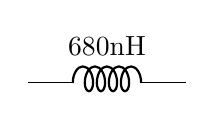
\begin{tikzpicture}
            \draw (0,0) to[L, label=680nH] ++(2,0);
        \end{tikzpicture}
        \caption{Ideal inductor Model}
        \label{fig:inductor_l}
    \end{subfigure}%
    \begin{subfigure}[b]{.5\linewidth}
        \centering
        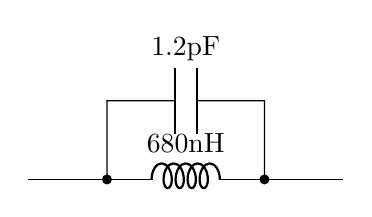
\begin{tikzpicture}
            \draw (0,0) to[L, label=680nH] ++(4,0);
            \draw (1, 0) to[short, *-] ++(0, 1)
            to[C, label=1.2pF] ++(2, 0)
            to[short, -*] ++(0, -1);
        \end{tikzpicture}
        \caption{Inductor with Parallel Capacitance}
        \label{fig:inductor_lc}
    \end{subfigure}%

    \begin{subfigure}[b]{.5\linewidth}
        \centering
        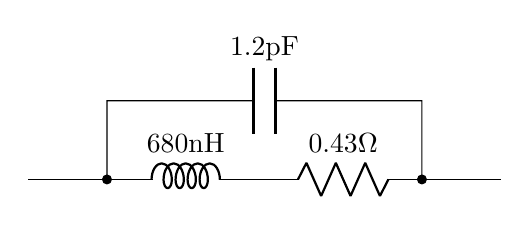
\begin{tikzpicture}
            \draw (0,0) to[short] ++(1,0)
            to[L, label=680nH] ++(2,0)
            to[R, label=$0.43\Omega$] ++(2,0)
            to[short] ++(1, 0);
            \draw (1, 0) to[short, *-] ++(0, 1)
            to[C, label=1.2pF] ++(4, 0)
            to[short, -*] ++(0, -1);
        \end{tikzpicture}
        \caption{Inductor Model with Additional Series Resistance}
        \label{fig:inductor_lcr}
    \end{subfigure}%
    \begin{subfigure}[b]{.5\linewidth}
        \centering
        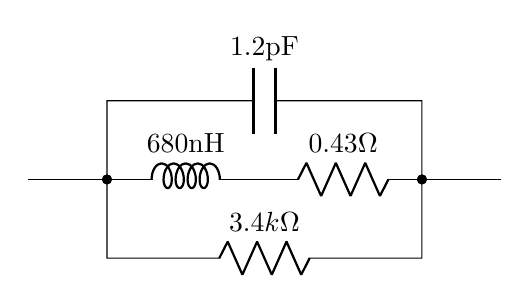
\begin{tikzpicture}
            \draw (0,0) to[short] ++(1,0)
            to[L, label=680nH] ++(2,0)
            to[R, label=$0.43\Omega$] ++(2,0)
            to[short] ++(1, 0);
            \draw (1, 0) to[short, *-] ++(0, 1)
            to[C, label=1.2pF] ++(4, 0)
            to[short, -*] ++(0, -1);
            \draw (1, 0) to[short, *-] ++(0, -1)
            to[R, label=$3.4k\Omega$] ++(4, 0)
            to[short, -*] ++(0, 1);
        \end{tikzpicture}
        \caption{Inductor Model with Additional Parallel Resistance}
        \label{fig:inductor_lcrr}
    \end{subfigure}%
    \caption{Electric Models of Real Life inductor}
\end{figure}

\begin{figure}
    \centering
    \begin{subfigure}{\linewidth}
        \centering
        \includegraphics[width=\linewidth]{./pics/inductor_models_smith.png}
        \caption{S11 of electric models of Inductor on Smith Chart}
        \label{fig:inductor_compare_s}
    \end{subfigure}

    \begin{subfigure}{\linewidth}
        \centering
        \includegraphics[width=\linewidth]{./pics/inductor_models_db.png}
        \caption{Magnitude of Impedance of electric models of Inductor in dBOhms}
        \label{fig:inductor_compare_z}
    \end{subfigure}
    \caption{Electric Characteristics of real inductor compared with various models}
    \label{fig:inductor_compare}
\end{figure}

\subsubsection{Ideal Inductor Model}

Using the impedance at 10MHz, we see that the inductance is roughly
$$\frac{42\Omega}{2\pi\cdot 10MHz \cdot 157 \Omega} \approx 670nH .$$
This is fairly close to the standard inductance value of $680nH$.
So our first model of the element would just be an ideal inductor of $680nH$ (\Cref{fig:inductor_l}).

The circuit is simulated in LTSpice and results are shown in \Cref{fig:inductor_compare}.
However, immediately we see that the ideal inductor does not fully characterize the real inductor.
In the Smith chart (\Cref{fig:inductor_compare_s}), the measured S11 crosses the real axis and goes into the lower half of the unit circle, and in the impedance magnitude plot (\Cref{fig:inductor_compare_z}), the measured impedance has a maximum at around 170MHz.


\subsubsection{Parallel Capacitance}
Since the measured impedance of the inductor goes down beyond 170MHz, this indicates the existence of some parasitic capacitance.
In an inductor, the closely based windings can act like capacitors, thus introducing some parallel capacitance (\Cref{fig:inductor_lc}).

The maximum impedance occurs at roughly 178MHz (which corresponds to S11 crossing the real axis).
This indicates that the 178MHz is the resonance frequency of the parallel LC circuit.
So the parallel capacitance can be calculated as
\[
    C = \frac{1}{(2\pi f)^2 L}
    = \frac{1}{(2\pi 178MHz)^2 \cdot 680nH}
    \approx
    1.2pF.
\]
As seen in \Cref{fig:inductor_compare}, the parallel LC model correctly predicts a maximum in the magnitude of the impedance around 178MHz, and the crossing of the real axis by the s parameter.

\subsubsection{Series Resistance}
However, as evident in \Cref{fig:inductor_compare_z}, the parallel LC model has a much higher Q than the actual inductor.

To lower the Q value, we should add some resistance.
The inductor is a big coil of wires that naturally have some resistance;
so we update our model to include that (\Cref{fig:inductor_lcr}).
Note that the series resistance is still parallel with the capacitance, since otherwise we would still have infinite impedance at resonance.

The value of the series resistance can be taken to be the real part of the impedance at low frequencies, when the inductor behaves like a short and the capacitor behaves like an open.
So we set series resistance to $0.43\Omega$.

The LTSpice simulated results are shown in \Cref{fig:inductor_compare}, and we can see that introduction of series impedance hardly reduced the Q value at all.

So we see that there must be some other important parasitics that we have not considered.

\subsubsection{Parallel Resistance}

A far smaller impedance than expected at resonance frequency suggests that we should consider adding some parallel resistance (\Cref{fig:inductor_lcrr}).
Its value can be taken to be the real part of the impedance at resonance, where the parallel $L$ and $C$ parts approximately represent a short.
So we set parallel resistance to $3.4k\Omega$.

As we can see from the results in \Cref{fig:inductor_compare_z}, adding this parallel resistance can make the model match the impedance maximum at around 178MHz very well;
and as shown in \Cref{fig:inductor_compare_s}, this even produces a better match at lower frequencies around $0\Omega$ than without the parallel resistance.

\subsubsection{Other Parasitics}
Our above model of the inductor still diverges from the measured inductor in that at higher frequencies -- the measured impedance magnitude is bigger than what the model predicts.
Naively, this would suggest that the parallel capacitance should be smaller.
However, changing the capacitance would also move the resonance frequency away from the expected value at 178MHz.
So we need to investigate other parasitics correctly explain this discrepancy.

\section{Summary}
In this lab we used VNA and LTSpice to build electric models that describe a capacitor and inductor.
We discovered that the capacitor can be pretty well described by a capacitor, an inductor, and a resistor in series; but the inductor needs a parallel capacitor, some series resistance, as well as some parallel resistance to model well.
Surprisingly, the parallel resistance of the inductor is quite small -- only $3.4k\Omega$.

This work can be extended by better understanding the residual parasitics of these components, as well as automating the process of building electric models for passive components.

\end{document}